\subsection{COINES C functions}\label{CoinesCFunctions}
\subsubsection{coinesAPI calls: Interface and board information}

\paragraph{coines\_open\_comm\_intf}
Opens the communication interface.

\begin{lstlisting}
int16_t coines_open_comm_intf(enum coines_comm_intf intf_type,void *arg); 
\end{lstlisting}

In case of MCU Target, API waits indefinitely for serial port or BLE connection (\texttt{MCU\_APP30} target and \texttt{MCU\_APP31} target).

In case of PC Target, one can configure communication settings either by passing the address of \texttt{coines\_serial\_com\_config} or \texttt{ble\_peripheral\_info} to \texttt{*arg}.

Serial\ com\ configuration:
\newline If \texttt{*arg} is NULL for \texttt{COINES\_COMM\_INTF\_USB}, first com port enumerated will be used for communication.
The serial com configuration structure contains the following items. Refer to \ref{serialComConfig} for its implementation.

\begin{lstlisting}
struct coines_serial_com_config
{
	uint32_t baud_rate; /*< Baud rate */
	uint16_t vendor_id; /*< vendor Id */
	uint16_t product_id; /*< Product Id */
	char* com_port_name; /*< serial com port name */
	uint16_t rx_buffer_size; /*< RX response buffer size */
};
\end{lstlisting}

BLE\ com\ configuration:
\newline If \texttt{*arg} is NULL for \texttt{COINES\_COMM\_INTF\_BLE}, the nearest Application board for the host BLE will be used for communication.
The ble com configuration structure contains the following items. Refer to \ref{bleComConfig} for its implementation.

\begin{lstlisting}
struct ble_peripheral_info
{
	char ble_address[COINES_CHAR_MAX_LEN]; /*< BLE device address */
	char ble_identifier[COINES_CHAR_MAX_LEN]; /*< BLE device identifier */
};
\end{lstlisting}

\paragraph{coines\_close\_comm\_intf}
Closes the communication interface.

\begin{lstlisting}
int16_t coines_close_comm_intf(enum coines_comm_intf intf_type,void *arg); 
\end{lstlisting}

\paragraph{coines\_get\_board\_info}
Gets the board information.

\begin{lstlisting}
int16_t coines_get_board_info(struct coines_board_info *data);
\end{lstlisting}

The data structure contains the following items 

\begin{lstlisting}
struct coines_board_info {
	/*!Board hardware ID */
	uint16_t hardware_id;
	/*!Board software ID */
	uint16_t software_id;
	/*!Type of the board like APP2.0, Arduino Due*/
	uint8_t board;
	/*!Shuttle ID of the sensor connected*/
	uint16_t shuttle_id;
};
\end{lstlisting}

\subsubsection{coinesAPI calls: GPIO oriented calls}

\paragraph{coines\_set\_pin\_config}
Sets the pin direction and the state.

\begin{lstlisting}
int16_t coines_set_pin_config(enum coines_multi_io_pin pin_number, enum coines_pin_direction direction, enum coines_pin_value pin_value);  
\end{lstlisting}

\paragraph{coines\_get\_pin\_config}
Gets the pin configuration.

\begin{lstlisting}
int16_t coines_get_pin_config(enum coines_multi_io_pin pin_number, enum coines_pin_direction *pin_direction, enum coines_pin_value *pin_value);
\end{lstlisting}

\paragraph{coines\_set\_shuttleboard\_vdd\_vddio\_config}
Configures the VDD and VDDIO of the sensor. For APP2.0, a voltage level of 0 or 3300 mV is supported. Any values above 0 will default to 3300 mV.

\begin{lstlisting}
int16_t coines_set_shuttleboard_vdd_vddio_config(uint16_t vdd_millivolt, uint16_t vddio_millivolt);
\end{lstlisting}

\subsubsection{coinesAPI calls: Sensor communication}

\paragraph{coines\_config\_i2c\_bus}
Configures the I\textsuperscript{2}C bus. 

\begin{lstlisting}
int16_t coines_config_i2c_bus(enum coines_i2c_bus bus, enum coines_i2c_mode i2c_mode);
\end{lstlisting}

The first argument refers to the bus on the board. Currently, on APP2.0, there is only one bus available, so the argument is always COINES\_I2C\_BUS\_0.

The following I\textsuperscript{2}C modes are available:
\begin{lstlisting}
COINES_I2C_STANDARD_MODE
COINES_I2C_FAST_MODE
COINES_I2C_SPEED_3_4_MHZ
COINES_I2C_SPEED_1_7_MHZ
\end{lstlisting}

\paragraph{coines\_config\_spi\_bus}
Configures the SPI bus of the board. The argument coines\_spi\_bus refers to the bus on the board. On APP2.0, there is only one bus available, so the user should only use COINES\_SPI\_BUS\_0. The SPI speed can be chosen in various discrete steps, as defined in enum coines\_spi\_speed in coines.h. (For example, COINES\_SPI\_SPEED\_2\_MHZ sets the SPI speed to 2 MHz.)

\begin{lstlisting}
int16_t coines_config_spi_bus(enum coines_spi_bus bus, uint32_t spi_speed, enum coines_spi_mode spi_mode);
\end{lstlisting}

\paragraph{coines\_config\_i2s\_bus}
This API is used to configure the I\textsuperscript{2}S bus to match the TDM configuration

\begin{lstlisting}
int16_t coines_config_i2s_bus(uint16_t data_words, coines_tdm_callback callback);
\end{lstlisting}

Arguments:
\begin{itemize}
	\item \texttt{data\_words}: number of words to use in the buffer. Max is set at COINES\_TDM\_BUFFER\_SIZE\_WORDS.
	\item \texttt{callback}: register a callback to be called to process and copy the data.
\end{itemize}

\paragraph{coines\_deconfig\_spi\_bus}
This API is used to de-configure the SPI bus

\begin{lstlisting}
int16_t coines_deconfig_spi_bus(enum coines_spi_bus bus);
\end{lstlisting}

\paragraph{coines\_deconfig\_i2c\_bus}
This API is used to de-configure the I\textsuperscript{2}C bus

\begin{lstlisting}
int16_t coines_deconfig_i2c_bus(enum coines_i2c_bus bus);
\end{lstlisting}

\paragraph{coines\_deconfig\_i2s\_bus}
This API is used to stop the I\textsuperscript{2}S/TDM interface from reading data from the sensor

\begin{lstlisting}
void coines_deconfig_i2s_bus(void);
\end{lstlisting}

\paragraph{coines\_write\_i2c}\label{CoinesWriteI2c}
Writes 8-bit register data to the I\textsuperscript{2}C device at \texttt{COINES\_I2C\_BUS\_0}.

\begin{lstlisting}
int8_t coines_write_i2c(enum coines_i2c_bus bus,uint8_t dev_addr, uint8_t reg_addr, uint8_t *reg_data, uint16_t count);
\end{lstlisting}

Arguments:
\begin{itemize}
	\item \texttt{bus}: I\textsuperscript{2}C bus to be used
	\item \texttt{dev\_addr}: I\textsuperscript{2}C device address.
	\item \texttt{reg\_addr}: Starting address for writing the data.
	\item \texttt{reg\_data}: Data to be written.
	\item \texttt{count}: Number of bytes to write.
\end{itemize}

\paragraph{coines\_read\_i2c}\label{CoinesReadI2c}
Reads 8-bit register data from the I\textsuperscript{2}C device at \texttt{COINES\_I2C\_BUS\_0}.

\begin{lstlisting}
int8_t coines_read_i2c(enum coines_i2c_bus bus,uint8_t dev_addr, uint8_t reg_addr, uint8_t *reg_data, uint16_t count);
\end{lstlisting}

Arguments:
\begin{itemize}
	\item \texttt{bus}: I\textsuperscript{2}C bus to be used
	\item \texttt{dev\_addr}: I\textsuperscript{2}C device address.
	\item \texttt{reg\_addr}: Starting address for reading the data.
	\item \texttt{reg\_data}: Buffer to take up the read data.
	\item \texttt{count}: Number of bytes to read.
\end{itemize}

\paragraph{coines\_i2c\_set}
This API is used to write the data in I2C communication.

\begin{lstlisting}
int8_t coines_i2c_set(enum coines_i2c_bus bus, uint8_t dev_addr, uint8_t *data, uint8_t count);
\end{lstlisting}

Arguments:
\begin{itemize}
	\item \texttt{bus}: I\textsuperscript{2}C bus to be used
	\item \texttt{dev\_addr}: I\textsuperscript{2}C device address.
	\item \texttt{data}: Data to be written.
	\item \texttt{count}: Number of bytes to write.
\end{itemize}

\paragraph{coines\_i2c\_get}
This API is used to read the data in I2C communication.

\begin{lstlisting}
int8_t coines_i2c_get(enum coines_i2c_bus bus, uint8_t dev_addr, uint8_t *data, uint8_t count);
\end{lstlisting}

Arguments:
\begin{itemize}
	\item \texttt{bus}: I\textsuperscript{2}C bus to be used
	\item \texttt{dev\_addr}: I\textsuperscript{2}C device address.
	\item \texttt{data}: Data read from the sensor.
	\item \texttt{count}: Number of bytes to read.
\end{itemize}

\paragraph{coines\_write\_spi}\label{CoinesWriteSpi}
Writes 8-bit register data to the SPI device at \texttt{COINES\_SPI\_BUS\_0}.

\begin{lstlisting}
int8_t coines_write_spi(enum coines_spi_bus bus,uint8_t dev_addr, uint8_t reg_addr, uint8_t *reg_data, uint16_t count);
\end{lstlisting}

Arguments:
\begin{itemize}
	\item \texttt{bus}: SPI bus to be used.
	\item \texttt{dev\_addr}: Chip select pin number.
	\item \texttt{reg\_addr}: Starting address for writing the data.
	\item \texttt{reg\_data}: Data to be written.
	\item \texttt{count}: Number of bytes to write.
\end{itemize}

\paragraph{coines\_read\_spi}\label{CoinesReadSpi}
Reads 8-bit register data from the SPI device at \texttt{COINES\_SPI\_BUS\_0}.

\begin{lstlisting}
int8_t coines_read_spi(enum coines_spi_bus bus,uint8_t dev_addr, uint8_t reg_addr, uint8_t *reg_data, uint16_t count);
\end{lstlisting}

Arguments:
\begin{itemize}
	\item \texttt{bus}: SPI bus to be used.
	\item \texttt{dev\_addr}: Chip select pin number.
	\item \texttt{reg\_addr}: Starting address for reading the data.
	\item \texttt{reg\_data}: Buffer to take up the read data.
	\item \texttt{count}: Number of bytes to read.
\end{itemize}

\paragraph{coines\_delay\_msec}
Introduces delay in millisecond.

\begin{lstlisting}
void coines_delay_msec(uint32_t delay_ms);
\end{lstlisting}

\paragraph{coines\_delay\_usec}
Introduces delay in microsecond.

\begin{lstlisting}
void coines_delay_usec(uint32_t delay_us);
\end{lstlisting}

\paragraph{coines\_uart\_init}
This API is used to initialize the UART communication

\begin{lstlisting}
int8_t coines_uart_init(enum coines_uart_instance uart_instance, enum coines_uart_parity parity, enum coines_uart_flow_control flow_control, uint32_t baud_rate);
\end{lstlisting}

Arguments:
\begin{itemize}
	\item \texttt{uart\_instance}: Specifies the UART instance
	\item \texttt{parity}: UART parity
	\item \texttt{flow\_control}: UART flow control mode
	\item \texttt{baud\_rate}:  UART baud rate
\end{itemize}

\paragraph{coines\_uart\_read}
This API is used to read the data in UART communication

\begin{lstlisting}
uint16_t coines_uart_read(enum coines_uart_instance uart_instance, uint8_t *buffer, uint16_t length);
\end{lstlisting}

Arguments:
\begin{itemize}
	\item \texttt{uart\_instance}: Specifies the UART instance
	\item \texttt{buffer}: Pointer to the buffer to store the data
	\item \texttt{length}: Length of the buffer
\end{itemize}

\paragraph{coines\_uart\_write}
This API is used to write the data in UART communication

\begin{lstlisting}
int8_t coines_uart_write(enum coines_uart_instance uart_instance, uint8_t *buffer, uint16_t length);
\end{lstlisting}

Arguments:
\begin{itemize}
	\item \texttt{uart\_instance}: Specifies the UART instance
	\item \texttt{buffer}: Pointer to the data buffer which need to be written
	\item \texttt{length}: Length of the buffer
\end{itemize}

\subsubsection{coinesAPI calls: Streaming feature}

Note :
\begin{enumerate}
\item The below APIs are supported only on PC Target.
\item A simpler approach of using \texttt{coines\_attach\_interrupt()} API for is available for MCU.
\end{enumerate}


\paragraph{coines\_config\_streaming}
Sets the configuration for streaming sensor data.

\begin{lstlisting}
int16_t coines_config_streaming(uint8_t channel_id, struct coines_streaming_config *stream_config, struct coines_streaming_blocks *data_blocks); 
\end{lstlisting}

Arguments:
\begin{itemize}
\item \texttt{channel\_id}: An integer number that can be used as identifier/index to the sensor data that will be streamed for this setting

\item \texttt{stream\_config}: Contains information regarding interface settings and streaming configuration.
\item  \texttt{coines\_streaming\_blocks}: Contains information regarding numbers of blocks to read, register address and size for each block.
\end{itemize}
Note:\newline
The below parameters should always be set:
	\begin{itemize}
		\item \texttt{data\_block.no\_of\_blocks}: number of blocks to stream (must at least be one)
		\item For each block b:
		\begin{itemize}
			\item \texttt{data\_block.reg\_start\_addr[b]}: start address of the block in the register map
			\item \texttt{stream\_block.no\_of\_data\_bytes[b]}: number of bytes to read, starting from the start address
		\end{itemize}
	\end{itemize}

For reading data from I\textsuperscript{2}C bus,then set the below parameters:
	
	\begin{itemize}
		\item \texttt{stream\_config.intf = COINES\_SENSOR\_INTF\_I2C;}
		\item \texttt{stream\_config.i2c\_bus}: I\textsuperscript{2}C bus (in case of APP2.0, this is always \texttt{COINES\_I2C\_BUS\_0})
		\item \texttt{stream\_config.dev\_addr}: I\textsuperscript{2}C address of the sensor
	\end{itemize}
For reading data from SPI bus, then set the below parameters:
	\begin{itemize}
		\item \texttt{stream\_config.intf = COINES\_SENSOR\_INTF\_SPI;}
		\item \texttt{stream\_config.spi\_bus}: SPI bus (in case of APP2.0, this is always \texttt{COINES\_SPI\_BUS\_0})
		\item \texttt{stream\_config.cs\_pin}: CS pin of the sensor, information can be obtained from the shuttle board documentation for the sensor. 
	\end{itemize}
When polling mode is requested, set the below parameters:
	\begin{itemize}
		\item \texttt{stream\_config.sampling\_units}: \\ either milliseconds (\texttt{COINES\_SAMPLING\_TIME\_IN\_MILLI\_SEC}) \\ or microseconds (\texttt{COINES\_SAMPLING\_TIME\_IN\_MICRO\_SEC})
		\item \texttt{stream\_config.sampling\_time}: sampling period in the unit as defined in \\ \texttt{stream\_config.sampling\_units}
	\end{itemize}
When interrupt mode is requested, set the below parameters:
	\begin{itemize}
		\item \texttt{stream\_config.int\_pin}: pin of the interrupt which shall trigger the sensor read-out. If the interrupt output of the sensor is used, the required information about the pin number can be obtained from the shuttle board documentation for the sensor.
		\item \texttt{stream\_config.int\_timestamp}:  it can be configured if the sensor data is tagged with a timestamp (\texttt{COINES\_TIMESTAMP\_ENABLE}) or not (\texttt{COINES\_TIMESTAMP\_DISABLE}).
	\end{itemize}

\paragraph{coines\_start\_stop\_streaming}
Starts or stops sensor data streaming.

\begin{lstlisting}
int16_t coines_start_stop_streaming(enum coines_streaming_mode stream_mode, uint8_t start_stop);
\end{lstlisting}

Arguments:
\begin{itemize}
	\item \texttt{stream\_mode}: streaming mode (either \texttt{COINES\_STREAMING\_MODE\_POLLING} or \\ \texttt{COINES\_STREAMING\_MODE\_INTERRUPT})
	\item \texttt{start\_stop}: flag to either start (\texttt{COINES\_STREAMING\_START}) or stop (\texttt{COINES\_STREAMING\_STOP}) the streaming
\end{itemize}

\paragraph{coines\_read\_stream\_sensor\_data}\label{coinesReadStreamSensorData}
Reads the data streamed from the sensor.

\begin{lstlisting}
int16_t coines_read_stream_sensor_data(uint8_t sensor_id, uint32_t number_of_samples, uint8_t *data, uint32_t *valid_samples_count);
\end{lstlisting}

Arguments:
\begin{itemize}
	\item \texttt{sensor\_id}: id of the sensor 
	\item \texttt{number\_of\_samples}: number of samples the user wishes to read (not implemented)
	\item \texttt{data}: data buffer
	\begin{itemize} 
	   \item Interrupt streaming - Packet counter + Register data + Timestamp
	   \item Polling streaming - Register data
	\end{itemize}
	\item \texttt{valid\_samples\_count}: number of samples the user has actually received (may be less than \texttt{number\_of\_samples})
\end{itemize}

Example of a packet:

\begin{figure}[h]
	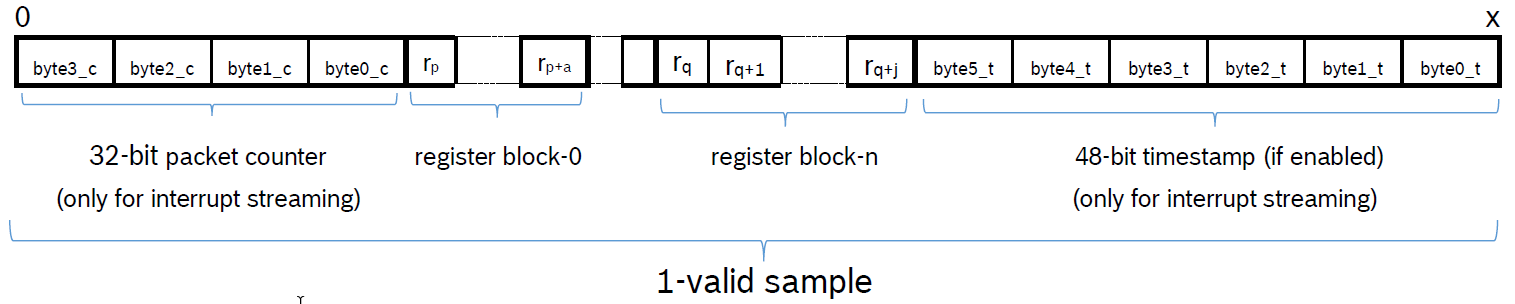
\includegraphics[width=\textwidth]{coinesAPI_images/COINES_streamingSample}
	\caption{Format of streaming packages}
\end{figure}

In the above figure, the following meaning apply to the mentioned abreviations:
\begin{itemize}
	\item r\textsubscript{p}: Value at register address p
	\item a: Size of register block–0
	\item r\textsubscript{p+a}: Value at register address p
\end{itemize}

Similarly is the case for r\textsubscript{q}, j and r\textsubscript{q+j}. See the \texttt{coines\_streaming\_blocks} structure for information regarding register blocks.

The packet counter and the timestamp can be obtained as follows:

\begin{itemize}
	\item[] \texttt{packet\_counter = (byte3\_c << 24) | (byte2\_c << 16) | (byte1\_c << 8) | (byte0\_c)}
	\item[] \texttt{timestamp = (byte5\_t << 40) | (byte4\_t << 32) | (byte3\_t << 24) | (byte2\_t << 16) | (byte1\_t << 8) | (byte0\_t)}
\end{itemize}

The 48-bit timestamp is enabled by using \\ \texttt{coines\_trigger\_timer(COINES\_TIMER\_START,  COINES\_TIMESTAMP\_ENABLE);}

Timestamp in microseconds can be obtained using below formula:
\begin{itemize}
	\item[] $\displaystyle Timestamp\ (\mu s) = \frac{48bit\_timestamp}{30}$
\end{itemize}

\paragraph{coines\_trigger\_timer}
Triggers the timer in firmware and also enables or disables the time stamp feature.

\begin{lstlisting}
int16_t coines_trigger_timer(enum coines_timer_config tmr_cfg,enum coines_time_stamp_config ts_cfg);
\end{lstlisting}

Arguments:
\begin{itemize}
	\item \texttt{tmr\_cfg}: start, stop or reset the timer (\texttt{COINES\_TIMER\_START}, \texttt{COINES\_TIMER\_STOP} or \\ \texttt{COINES\_TIMER\_RESET}) 
	\item \texttt{ts\_cfg}: Enables/disables microcontroller timestamp  (\texttt{COINES\_TIMESTAMP\_ENABLE} or \\ \texttt{COINES\_TIMESTAMP\_DISABLE}) 
\end{itemize}

\subsubsection{coinesAPI calls: Other useful APIs}
\paragraph{coines\_get\_millis}
Returns the number of milliseconds passed since the program started

\begin{lstlisting}
uint32_t coines_get_millis();
\end{lstlisting}

\paragraph{coines\_get\_micro\_sec}
Returns the number of microseconds passed since the program started

\begin{lstlisting}
uint64_t coines_get_micro_sec();
\end{lstlisting}

\paragraph{coines\_attach\_interrupt}
Attaches an interrupt to a Multi-IO pin.Works only on MCU.

\begin{lstlisting}
void coines_attach_interrupt(enum coines_multi_io_pin pin_number,void (*callback)(uint32_t, uint32_t),enum coines_pin_interrupt_mode int_mode);
\end{lstlisting}

Arguments:
\begin{itemize}
	\item \texttt{pin\_number}:  Multi-IO pin
	\item \texttt{callback}: Name of the function to be called on detection of interrupt
	\item \texttt{int\_mode}: Trigger modes - change (\texttt{COINES\_PIN\_INTERRUPT\_CHANGE}), \\
	rising edge (\texttt{COINES\_PIN\_INTERRUPT\_RISING\_EDGE}), \\falling edge (\texttt{COINES\_PIN\_INTERRUPT\_FALLING\_EDGE})
\end{itemize}

\paragraph{coines\_detach\_interrupt}
Detaches interrupt from a Multi-IO pin.Works only on MCU.

\begin{lstlisting}
void coines_detach_interrupt(enum coines_multi_io_pin pin_number);
\end{lstlisting}

Arguments:
\begin{itemize}
	\item \texttt{pin\_number}: Multi-IO pin.
\end{itemize}

\paragraph{coines\_intf\_available}
Return the number of bytes available in the read buffer of the interface.Works only on APP3.x MCU target.

\begin{lstlisting}
uint16_t coines_intf_available(enum coines_comm_intf intf);
\end{lstlisting}

Arguments:
\begin{itemize}
	\item \texttt{intf}: Type of interface (USB, COM, or BLE)
\end{itemize}

\paragraph{coines\_intf\_connected}
Check if the interface is connected.Works only on APP3.x MCU target.

\begin{lstlisting}
bool coines_intf_connected(enum coines_comm_intf intf);
\end{lstlisting}

Arguments:
\begin{itemize}
	\item \texttt{intf}: Type of interface (USB, COM, or BLE)
\end{itemize}

\paragraph{coines\_flush\_intf}
Flush the write buffer.Works only on APP3.x MCU target.

\begin{lstlisting}
void coines_flush_intf(enum coines_comm_intf intf);
\end{lstlisting}

Arguments:
\begin{itemize}
	\item \texttt{intf}: Type of interface (USB, COM, or BLE)
\end{itemize}

\paragraph{coines\_read\_intf}
Read data over the specified interface.Works only on APP3.x MCU target.

\begin{lstlisting}
uint16_t coines_read_intf(enum coines_comm_intf intf, void *buffer, uint16_t len);
\end{lstlisting}

Arguments:
\begin{itemize}
	\item \texttt{intf}: Type of interface (USB, COM, or BLE)
	\item \texttt{buffer}: Pointer to the buffer to store the data
	\item \texttt{len}: Length of the buffer
\end{itemize}

\paragraph{coines\_write\_intf}
Write data over the specified interface.Works only on APP3.x MCU target.

\begin{lstlisting}
uint16_t coines_write_intf(enum coines_comm_intf intf, void *buffer, uint16_t len);
\end{lstlisting}

Arguments:
\begin{itemize}
	\item \texttt{intf}: Type of interface (USB, COM, or BLE)
	\item \texttt{buffer}: Pointer to the buffer storing the data
	\item \texttt{len}: Length of the buffer
\end{itemize}

\paragraph{coines\_get\_version}
Returns pointer to COINES version string

\begin{lstlisting}
char* coines_get_version(void);
\end{lstlisting}

\paragraph{coines\_soft\_reset}
Resets the device. After reset device jumps to the address specified in makefile(APP\_START\_ADDRESS).

\begin{lstlisting}
void coines_soft_reset(void);
\end{lstlisting}

\paragraph{coines\_read\_temp\_data}
This API is used to read the temperature sensor data.

\begin{lstlisting}
int16_t coines_read_temp_data(float *temp_data);
\end{lstlisting}
        
Arguments:
\begin{itemize}
	\item \texttt{temp\_conv\_data}: Buffer to retrieve the sensor data in degree Celsius.
\end{itemize}

\paragraph{coines\_read\_bat\_status}
This API is used to read the battery status.

\begin{lstlisting}
int16_t coines_read_bat_status(uint16_t *bat_status_mv, uint8_t *bat_status_percent);
\end{lstlisting}

Arguments:
\begin{itemize}
	\item \texttt{bat\_status\_mv}: Buffer to retrieve the battery status in millivolt
	\item \texttt{bat\_status\_percent}: Buffer to retrieve the battery status in percentage
\end{itemize}

\paragraph{coines\_ble\_config}
This API is used to configure BLE name and power. It should be called before calling coines\_open\_comm\_intf API.

\begin{lstlisting}
int16_t coines_ble_config(struct coines_ble_config *ble_config);
\end{lstlisting}

Arguments:
\begin{itemize}
	\item \texttt{ble\_config}: structure holding ble name and power details
\end{itemize}

\paragraph{coines\_set\_led}
 This API is used to set led state(on or off).
 
\begin{lstlisting}
int16_t coines_set_led(enum coines_led led,enum coines_led_state led_state);
\end{lstlisting}

Arguments:
\begin{itemize}
	\item \texttt{led}: led to which the state has to be set.
	\item \texttt{led\_state}: state to be set to the given led.
\end{itemize}

\paragraph{coines\_timer\_config}
 This API is used to configure the hardware timer.
 
\begin{lstlisting}
int16_t coines_timer_config(enum coines_timer_instance instance, void* handler);
\end{lstlisting}

Arguments:
\begin{itemize}
	\item \texttt{instance}: timer instance.
	\item \texttt{handler}: callback to be called when timer expires.
\end{itemize}

\paragraph{coines\_timer\_deconfig}
 This API is used to de-configure the hardware timer.
 
\begin{lstlisting}
int16_t coines_timer_deconfig(enum coines_timer_instance instance);
\end{lstlisting}

Arguments:
\begin{itemize}
	\item \texttt{instance}: timer instance.
\end{itemize}

\paragraph{coines\_timer\_start}
 This API is used to start the configured hardware timer.
 
\begin{lstlisting}
int16_t coines_timer_start(enum coines_timer_instance instance, uint32_t timeout);
\end{lstlisting}

Arguments:
\begin{itemize}
	\item \texttt{instance}: timer instance.
	\item \texttt{timeout}: timeout in microseconds.
\end{itemize}

\paragraph{coines\_timer\_stop}
 This API is used to stop the  hardware timer.
 
\begin{lstlisting}
int16_t coines_timer_stop(enum coines_timer_instance instance);
\end{lstlisting}

Arguments:
\begin{itemize}
	\item \texttt{instance}: timer instance.
\end{itemize}

\paragraph{coines\_get\_realtime\_usec}
This API is used to get the current counter(RTC) reference time in usec

\begin{lstlisting}
uint32_t coines_get_realtime_usec(void);
\end{lstlisting}

\paragraph{coines\_delay\_realtime\_usec}
This API is used to introduce delay based on high precision RTC(LFCLK crystal) with the resolution of 30.517 usec.

\begin{lstlisting}
void coines_delay_realtime_usec(uint32_t period);
\end{lstlisting}

Arguments:
\begin{itemize}
	\item \texttt{period}: required delay in microseconds 
\end{itemize}

\paragraph{coines\_attach\_timed\_interrupt}
Attaches a timed interrupt to a Multi-IO pin.

\begin{lstlisting}
int16_t coines_attach_timed_interrupt(enum coines_multi_io_pin pin_number, void (*timed_interrupt_cb)(uint64_t,uint32_t,uint32_t), enum coines_pin_interrupt_mode int_mode);
\end{lstlisting}

Arguments:
\begin{itemize}
	\item \texttt{pin\_number}: Multi-IO pin.
	\item \texttt{timed\_interrupt\_cb}: Name of the function to be called on detection of interrupt.
	\item \texttt{int\_mode}: Trigger modes - change,rising edge,falling edge.
\end{itemize}

\paragraph{coines\_detach\_timed\_interrupt}
Detaches a timed interrupt from a Multi-IO pin.

\begin{lstlisting}
int16_t coines_detach_timed_interrupt(enum coines_multi_io_pin pin_number);
\end{lstlisting}

Arguments:
\begin{itemize}
	\item \texttt{pin\_number}: Multi-IO pin.
\end{itemize}

\paragraph{coines\_echo\_test}
This API is used to test the communication.

\begin{lstlisting}
int16_t coines_echo_test(uint8_t *data, uint16_t length);
\end{lstlisting}

Arguments:
\begin{itemize}
	\item \texttt{data}: Data to be sent for testing.
	\item \texttt{length}: Length of the data.
\end{itemize}

\paragraph{coines\_shuttle\_eeprom\_write}
This API is used to write the content into shuttle eeprom.

\begin{lstlisting}
int16_t coines_shuttle_eeprom_write(uint16_t start_addr, uint8_t *buffer, uint16_t length);
\end{lstlisting}

Arguments:
\begin{itemize}
	\item \texttt{start\_addr}: EEPROM write address.
	\item \texttt{buffer}: Pointer to the buffer.
	\item \texttt{length}: Length of the buffer.
\end{itemize}

\paragraph{coines\_shuttle\_eeprom\_read}
This API is used to read the content from shuttle eeprom.

\begin{lstlisting}
int16_t coines_shuttle_eeprom_read(uint16_t start_addr, uint8_t *buffer, uint16_t length);
\end{lstlisting}

Arguments:
\begin{itemize}
	\item \texttt{start\_addr}: EEPROM read address.
	\item \texttt{buffer}: Pointer to the buffer.
	\item \texttt{length}: Length of the buffer.
\end{itemize}

\paragraph{coines\_yield}
This API can be defined to perform a task when yielded from an ongoing blocking call.

\begin{lstlisting}
void coines_yield(void);
\end{lstlisting}

\paragraph{coines\_execute\_critical\_region}
This API is used to execute the function inside critical region.

\begin{lstlisting}
void coines_execute_critical_region(coines_critical_callback callback);
\end{lstlisting}

Arguments:
\begin{itemize}
	\item \texttt{callback}: function to execute.
\end{itemize}

\paragraph{coines\_scan\_ble\_devices}\label{coinesScanBleDevices}
This API is used to connect to BLE Adapter and return list of BLE peripherals found during BLE scan.

\begin{lstlisting}
	int8_t coines_scan_ble_devices(struct ble_peripheral_info *ble_info, uint8_t *peripheral_count, size_t scan_timeout_ms)
\end{lstlisting}

Arguments:
\begin{itemize}
	\item \texttt{ble\_info}: array of struct containing found BLE peripheral information
	\item \texttt{peripheral\_count}: number of BLE peripherals found
	\item \texttt{scan\_timeout\_ms}: timeout for BLE scan
\end{itemize}

\newpage
